\chapter{Higher group theory}
In this section I describe joint work with Ulrik Buchholtz and Floris van Doorn \cite{highergroups}.

\subsection{From RPn to higher groups}
\begin{defn}
For any type $X$, we define \define{the connected component of $X$ in $\UU$} to be the type \[\UU_X\defeq\sm{A:\UU}\brck{A=X}.\] In particular, we have the type \[\UU_{\sphere{0}}\jdeq\sm{A:\UU}\brck{A={\sphere{0}}}\] of $2$\nobreakdash-element sets.

An \define{$X$\nobreakdash-bundle} over a type $A$ is defined to be a type family $B:A\to\UU_X$. 
\end{defn}

A term of type $\UU_X$ is formally a pair of a small type $A:\UU$ together with a term of type $\brck{A=X}$, but since the latter is a mere proposition we usually omit it, and consider the term itself as a small type.

\section{The real projective spaces}
In this section I describe joint work with Ulrik Buchholtz \cite{realprojective}, in which we defined the real projective spaces $\rprojective{n}$ in homotopy type theory. Furthermore, I answer a question posed by André Joyal during his visit of CMU in February 2018, regarding the complement of the tautological bundle on $\rprojective{n}$.

\subsection{The type of $2$-element sets}
\begin{thm}\label{thm:ptd_2elt_sets}
The type
\begin{equation*}
\sm{A:\UU_{\sphere{0}}}A
\end{equation*}
of pointed $2$\nobreakdash-element sets is contractible.
\end{thm}

\begin{proof}
We take $\pairr{\sphere{0},\north}$ as the center of contraction. We need to define
an identification of type $\pairr{\sphere{0},\north}=\pairr{A,a}$, 
for any $A:\UU_{\sphere{0}}$ and $a:A$. 

Let $A:\UU_{\sphere{0}}$ and $a:A$. By \autoref{lem:equiv_of_ptdtype}, we have
an equivalence of type
\begin{equation*}
\eqv{\Big(\pairr{\sphere{0},\north}=\pairr{A,a}\Big)}{\Big(\sm{e:\eqv{\sphere{0}}{A}}e(\north)=a\Big)}.
\end{equation*}
Hence we can complete the proof by constructing a term of type 
\begin{equation}\label{eq:Sn0_ptdequiv}
\sm{e:\eqv{\sphere{0}}{A}}e(\north)=a.
\end{equation} 

It is time for a little trick. Instead of constructing a term the type in
\autoref{eq:Sn0_ptdequiv}, we will show that this type is contractible.
Since being contractible is a mere proposition, 
this allows us to eliminate the assumption $\brck{\sphere{0}=A}$
into the assumption $p:\sphere{0}=A$. Note that the end point of $p$ is free.
Therefore we eliminate $p$ into $\refl{\sphere{0}}$. 
Thus, we see that it suffices to show that the type
\begin{equation*}
\sm{e:\eqv{\sphere{0}}{\sphere{0}}}e(\north)=a
\end{equation*}
is contractible for any $a:\sphere{0}$. 

This can be done by case analysis on $a:\sphere{0}$. Since we have the equivalence
$\bneg:\eqv{\sphere{0}}{\sphere{0}}$ that swaps $\north$ and $\south$, it follows
that $\sm{e:\eqv{\sphere{0}}{\sphere{0}}}e(\north)=\north$ is contractible if and only
if $\sm{e:\eqv{\sphere{0}}{\sphere{0}}}e(\north)=\south$ is contractible. Therefore, we
only need to show that the type
\begin{equation*}
\sm{e:\eqv{\sphere{0}}{\sphere{0}}}e(\north)=\north
\end{equation*}
is contractible. 
For the center of contraction we take $\pairr{\idfunc[\sphere{0}],\refl{\north}}$.
It remains to construct a term of type
\begin{equation*}
\prd{e:\eqv{\sphere{0}}{\sphere{0}}}{p:e(\north)=\north} \pairr{e,p}=\pairr{\idfunc[\sphere{0}],\refl{\north}}.
\end{equation*} 

Let $e:\eqv{\sphere{0}}{\sphere{0}}$ and $p:e(\north)=\north$.
By \autoref{lem:equiv_of_ptdequiv}, we have an equivalence of type
\begin{equation*}
\eqv{\Big(\pairr{e,p}=\pairr{\idfunc[\sphere{0}],\refl{\north}}\Big)}
    {\Big(\sm{h:e\htpy \idfunc[\sphere{0}]} p=h(\north)\Big)}.
\end{equation*}
Hence it suffices
to construct a term of the type on the right hand side.

We define a homotopy $h:e\htpy \idfunc[\sphere{0}]$ by case analysis: we take
$h(\north)\defeq p$. To define $h(\south)$, note that the type
$\hfib{e}{\south}$ is contractible. Therefore, we have a center of contraction
$\pairr{x,q}:\hfib{e}{\south}$. Recall that equality on $\sphere{0}$ is decidable,
so we have a term of type $(x=\north)+(x=\south)$. Since $e(\north)=\north$,
it follows that $\neg(x=\north)$. Therefore we have $x=\south$ and $e(x)=\south$.
It follows that $e(\south)=\south$, which we use to define $h(\south)$. 
\end{proof}

The main application we have in mind for \autoref{thm:ptd_2elt_sets}, is
a computation of the identity type of the type of $2$\nobreakdash-element sets, via
the encode-decode method, \autoref{lem:encode-decode}.

\begin{cor}\label{cor:id_U2}
The canonical map
\begin{equation*}
\mathsf{enc}_{{\sphere{0}},\north} : \prd*{A:\UU_{\sphere{0}}} ({\sphere{0}}= A)\to A
\end{equation*}
is an equivalence.
\end{cor}

Another way of stating the following theorem, is by saying that the map
$\unit\to\UU_{\sphere{0}}$ \emph{classifies} the ${\sphere{0}}$\nobreakdash-bundles.

\begin{thm}\label{lem:classifyer_U2}
Let $B:A\to\UU_{\sphere{0}}$ be a ${\sphere{0}}$\nobreakdash-bundle. Then the square
\begin{equation*}
\begin{tikzcd}
\sm{x:A}B(x) \arrow[r] \arrow[d,swap,"\proj 1"] & \unit \arrow[d,"{\sphere{0}}"] \\
A \arrow[r,swap,"B"] & \UU_{\sphere{0}}
\end{tikzcd}
\end{equation*}
commutes via a homotopy $R_{A,B}:\prd{x:A}{y:B(x)} \eqv{B(x)}{\sphere{0}}$, and is a pullback square. 
\end{thm}

\begin{proof}[Construction]
Since $B(x):\UU_{\sphere{0}}$ for any $x:A$, 
we have by \autoref{cor:id_U2} the fiberwise equivalence
\begin{equation*}
\mathsf{enc}_{\sphere{0},\N}(B(x)):\eqv{(\sphere{0}=B(x))}{B(x)}
\end{equation*} 
indexed by $x:A$. 
Hence it follows by Theorem 4.7.7 of \cite{hottbook} that the induced map
of total spaces is an equivalence. It follows that the diagram
\begin{equation*}
\begin{tikzcd}
\sm{x:A}B(x) \arrow[drr,bend left=15] \arrow[ddr,bend right=15,swap,"\proj 1"] \arrow[dr,densely dotted,"\eqvsym"] \\
& \sm{x:A} ({\sphere{0}}=B(x)) \arrow[r] \arrow[d,swap,"\proj 1"] & \unit \arrow[d,"{\lam{\nameless}\sphere{0}}"] \\
& A \arrow[r,swap,"B"] & \UU_{\sphere{0}}
\end{tikzcd}
\end{equation*}
commutes. Since the inner square is a pullback square, it follows that the outer square is a pullback square.
\end{proof}

\subsection{Finite dimensional real projective spaces}
\label{sec:fdrp}

Classically, the $(n+1)$-st real projective space can be obtained by attaching an $(n+1)$-cell to the $n$-th real projective space. This suggests a way of defining the real projective spaces that involves simultaneously defining $\rprojective{n}$ and an attaching map $\alpha_n : \sphere{n}\to\rprojective{n}$. Then we obtain $\rprojective{n+1}$ as the mapping cone of $\alpha_n$, i.e., as a pushout
\begin{equation*}
\begin{tikzcd}
\sphere{n} \arrow[r,"\alpha_n"] \arrow[d] & \rprojective{n} \arrow[d] \\
\unit \arrow[r] & \rprojective{n+1},
\end{tikzcd}
\end{equation*}
and we have to somehow find a way to define the attaching map $\alpha_{n+1}:\sphere{n+1}\to\rprojective{n}$ to continue the inductive procedure.
However, it is somewhat tricky to obtain these attaching maps directly, and we have chosen to follow a closely related path towards the definition of the real projective spaces that takes advantage of the machinery of dependent type theory. 

Observe that the attaching map $\alpha_n:\sphere{n}\to\rprojective{n}$ is just the tautological bundle (or the quotient map that identifies the antipodal points). This suggests that we may proceed by defining simultaneously the real projective space $\rprojective{n}$ and its tautological bundle $\tautfam[\R]{n}$. The tautological bundle on $\rprojective{n}$ is an $\sphere{0}$-bundle, so it can be described as a map $\rprojective{n}\to\UU_{\sphere{0}}$. We perform this construction in \autoref{defn:realprojective} using the properties of the type of 2-element types developed in \autoref{sec:UUS0}, and in \autoref{thm:Sn_totalcov} we show that the total space of the tautological bundle on $\rprojective{n}$ is the $n$-sphere. 

\begin{defn}\label{defn:realprojective}
We define simultaneously for each $n:\N_{-1}$, 
the \define{$n$-dimensional real projective space} $\rprojective{n}$, 
and the \define{tautological bundle} $\tautfam[\R]{n}:\rprojective{n}\to \UU_{\sphere{0}}$.
\end{defn}

\begin{proof}[Construction]
The construction is by induction on $n:\N_{-1}$.
For the base case $n\defeq -1$, 
we take $\rprojective{-1}\defeq\emptyt$. 
Then there is a unique map of type $\rprojective{-1}\to \UU_{\sphere{0}}$, which we
take as our definition of $\tautfam[\R]{-1}$.

For the inductive step, suppose $\rprojective{n}$ and $\tautfam[\R]{n}$ are defined. Then we define $\rprojective{n+1}$ to be the pushout
\begin{equation*}
\begin{tikzcd}
{\sm{x:\rprojective{n}}\tautfam[\R]{n}(x)} \arrow[d,swap,"\proj 1"] \arrow[r] & \unit \arrow[d,"\base"] \\
\rprojective{n} \arrow[r,swap,"\inr"] & \rprojective{n+1}
\end{tikzcd}
\end{equation*}
In other words, 
$\rprojective{n+1}$ is the \emph{mapping cone} of the tautological bundle, 
when we view the tautological bundle as the projection 
$\proj 1:(\sm{x:\rprojective{n}}\tautfam[\R]{n}(x))\to\rprojective{n}$. 

To define $\tautfam[\R]{n+1}:\rprojective{n+1}\to \UU_{\sphere{0}}$
we use the universal property of $\rprojective{n+1}$. 
Therefore, it suffices to show that the outer square in the diagram
\begin{equation}\label{eq:diagram}
\begin{tikzcd}
{\sm{x:\rprojective{n}}\tautfam[\R]{n}(x)} \arrow[d,swap,"\proj 1"] \arrow[r] & \unit \arrow[d,swap,"\base"] \arrow[ddr,bend left=15,"\sphere{0}"]\\
\rprojective{n} \arrow[drr,bend right=15,swap,"{\tautfam[\R]{n}}"] \arrow[r,swap,"\inr"] & \rprojective{n+1} \arrow[dr,densely dotted] \\
& & \UU_{\sphere{0}}
\end{tikzcd}
\end{equation}
commutes. Indeed, in \autoref{lem:classifyer_U2} we have constructed a homotopy 
\begin{equation*}
R_n\defeq R_{\rprojective{n},\tautfam[\R]{n}}:\prd{x:\rprojective{n}}{y:\tautfam[\R]{n}} \eqv{\tautfam[\R]{n}(x)}{\sphere{0}},
\end{equation*}
and in fact, this square is a pullback.
\end{proof}

\begin{eg}
We have $\rprojective{-1}=\emptyt$, $\rprojective{0}=\unit$, and $\rprojective{1}=\sphere{1}$. 
\end{eg}

\begin{thm}\label{thm:Sn_totalcov}
For each $n:\N_{-1}$, there is an equivalence
\begin{equation*}
e_n:\eqv{\sphere{n}}{\sm{x:\rprojective{n}}\tautfam[\R]{n}(x)}.
\end{equation*}
\end{thm}

In other words, $\rprojective{n+1}$ is obtained from $\rprojective{n}$ by attaching a single $(n+1)$\nobreakdash-disk, i.e., as a pushout
\begin{equation*}
\begin{tikzcd}
\sphere{n} \arrow[r] \arrow[d,swap,"\proj1\circ e_n"] & \unit \arrow[d] \\
\rprojective{n} \arrow[r] & \rprojective{n+1}.
\end{tikzcd}
\end{equation*}

\begin{proof}
For $n\jdeq -1$, we have $\rprojective{-1}\jdeq\emptyt$ and the unique tautological bundle $\tautfam[\R]{-1}$. Therefore the type $\sm{x:\rprojective{-1}}\tautfam[\R]{-1}(x)$ is equivalent to the empty type, which is $\sphere{-1}$ by definition. This gives the base case.

Now assume that we have an equivalence $e_n:\eqv{\sphere{n}}{\sm{x:\rprojective{n}}\tautfam[\R]{n}(x)}$. 
Our goal is to construct the equivalence
\begin{equation*}
e_{n+1}:\eqv{\sphere{n+1}}{\sm{x:\rprojective{n+1}}\tautfam[\R]{n+1}(x)}.
\end{equation*}
such that the square
\begin{equation}\label{eq:Sn_totalcov_natural}
\begin{tikzcd}
\sphere{n} \arrow[d,swap,"e_{n}"] \arrow[r,"\inl"] & \sphere{n+1} \arrow[d,"e_{n+1}"] \\
\sm{x:\rprojective{n}}\tautfam[\R]{n}(x) \arrow[r] & \sm{x:\rprojective{n+1}}\tautfam[\R]{n+1}(x)
\end{tikzcd}
\end{equation}
commutes. By the functoriality of the join (or equivalently, by equivalence induction on $e_n$), it suffices to find an equivalence
\begin{equation*}
\alpha:\eqv{\join{\Big(\sm{x:\rprojective{n}}\tautfam[\R]{n}(x)\Big)}{\sphere{0}}}{\sm{x:\rprojective{n+1}}\tautfam[\R]{n+1}(x)},
\end{equation*}
such that the bottom triangle in the diagram
\begin{equation*}
\begin{tikzcd}
\sphere{n} \arrow[r,"\inl"] \arrow[d,swap,"e_n"] & \sphere{n+1} \arrow[d,"\join{e_n}{\idfunc[\sphere{0}]}"] \\
\sm{x:\rprojective{n}}\tautfam[\R]{n}(x) \arrow[r,"\inl"] \arrow[dr] & \join{\Big(\sm{x:\rprojective{n}}\tautfam[\R]{n}(x)\Big)}{\sphere{0}} \arrow[d,"\alpha"] \\
& \sm{x:\rprojective{n+1}}\tautfam[\R]{n+1}(x)
\end{tikzcd}
\end{equation*}
commutes.
We construct this equivalence using the flattening lemma, \autoref{lem:flattening}, from which we get a pushout square:
\begin{equation*}
\begin{tikzcd}[column sep=0.5em]
\sm{x:\rprojective{n}}{y:\tautfam[\R]{n}(x)}\tautfam[\R]{n}(x) \arrow[r] \arrow[d] & \sm{t:\unit}\sphere{0} \arrow[d] \\
\sm{x:\rprojective{n}}\tautfam[\R]{n}(x) \arrow[r] & \sm{x:\rprojective{n+1}}\tautfam[\R]{n+1}(x)
\end{tikzcd}
\end{equation*}
We can calculate this pushout by constructing a natural transformation of spans (diagrams in $\UU$ of the form $\cdot\leftarrow\cdot\rightarrow\cdot$), as indicated by the diagram in Fig.~\ref{fig:sphere-equiv}.
\begin{figure*}
  \centering
\begin{tikzcd}[column sep=6em]
\sm{x:\rprojective{n}}\tautfam[\R]{n}(x) \arrow[d,swap,"\idfunc"]
  & \sm{x:\rprojective{n}}{y:\tautfam[\R]{n}(x)}\tautfam[\R]{n}(x) \arrow[l,swap,"\pairr{x,z}\mapsfrom\pairr{x,y,z}" yshift=1ex] \arrow[d,densely dotted,"u"] \arrow[r,"\pairr{x,y,z}\mapsto\pairr{\ttt,R_n(x,y,z)}" yshift=1ex] 
  & \sm{t:\unit}\sphere{0} \arrow[d,"\proj 2"] \\
\sm{x:\rprojective{n}}\tautfam[\R]{n}(x)
  &
\Big(\sm{x:\rprojective{n}}\tautfam[\R]{n}(x)\Big)\times\sphere{0} \arrow[l,"\pi_1"] \arrow[r,swap,"\pi_2"]
  & \sphere{0}
\end{tikzcd}
\caption{Map of spans used in the proof of Thm~\ref{thm:Sn_totalcov}. The map $u$ is given by $\pairr{x,y,z}\mapsto\pairr{x,z,R_n(x,y,z)}$.}
\label{fig:sphere-equiv}
\end{figure*}
To show that the map $u$ in Fig.~\ref{fig:sphere-equiv} is an equivalence, it suffices to show that $R_n(x,y,z)=R_n(x,y,z)$ for any $x$, $y$, and $z$, because then it follows that $u$ is homotopic to the total map of a fiberwise equivalence. More generally, it suffices to show that $R_{\UU_{\sphere{0}},T}(X,x,y)=R_{\UU_{\sphere{0}},T}(X,y,x)$, where $T$ is the tautological bundle on $\UU_{\sphere{0}}$. Since $\UU_{\sphere{0}}$ is connected and since our goal is a mere proposition, we only need to verify the claim at the base point $\sphere{0}$ of $\UU_{\sphere{0}}$. This boils down to verifying that the group multiplication of $\Zmodtwo$ is indeed commutative.
\end{proof}

\begin{cor}
We obtain the fiber sequence
\begin{equation*}
\begin{tikzcd}
\sphere{0} \arrow[r,hook] & \sphere{n} \arrow[r,->>] & \rprojective{n}.
\end{tikzcd}
\end{equation*}
Hence, for each $k\geq 2$ we have $\pi_k(\sphere{n})=\pi_k(\rprojective{n})$. 
\end{cor}

\begin{proof}
Since we have the double cover $\tautfam[\R]{n}:\rprojective{n}\to\UU_{\sphere{0}}$ with total space $\sphere{n}$, we obtain the long exact sequence
\begin{equation*}
\begin{tikzcd}
  \cdots \arrow[r]
  & \pi_{k+1}(\sphere{n}) \arrow[r] \arrow[d, phantom, ""{coordinate, name=Z}]
  & \pi_{k+1}(\rprojective n) \arrow[dll, rounded corners,
      to path={ -- ([xshift=8.5ex]\tikztostart.center)
                |- (Z) [near end]\tikztonodes
                -| ([xshift=-8ex]\tikztotarget.center) -- (\tikztotarget)}] \\
  \pi_k(\sphere{0}) \arrow[r]
  & \pi_k(\sphere{n}) \arrow[r] \arrow[d, phantom, ""{coordinate, name=W}]
  & \pi_k(\rprojective n) \arrow[dll, rounded corners,
      to path={ -- ([xshift=8.5ex]\tikztostart.center)
                |- (W) [near end]\tikztonodes
                -| ([xshift=-8ex]\tikztotarget.center) -- (\tikztotarget)}] \\
  \pi_{k-1}(\sphere{0}) \arrow[r]
  & \pi_{k-1}(\sphere{n}) \arrow[r]
  & \cdots
\end{tikzcd}
\end{equation*}
Since $\pi_k({\sphere{0}})=0$ for $k\geq 1$, we get the desired isomorphisms.
\end{proof}

\subsection{The infinite dimensional real projective space}
\label{sec:idrp}

Observe that from the definition of $\rprojective{n}$ and its tautological 
cover, we obtain a commutative diagram of the form:
\begin{equation*}
\begin{tikzcd}[row sep=large,column sep=large]
\rprojective{-1} \arrow[r,"\inr"] \arrow[dr,swap,"{\tautfam[\R]{-1}}"] 
& \rprojective{0} \arrow[d,swap,near start,"{\tautfam[\R]{0}}"] \arrow[r,"\inr"] 
& \rprojective{1} \arrow[dl,swap,"{\tautfam[\R]{1}}"] \arrow[r,"\inr"] 
& \cdots \arrow[dll,"{\tautfam[\R]{2}}"]\\
& \UU_{\sphere{0}}
\end{tikzcd}
\end{equation*}
Using this sequence, we define the infinite dimensional real projective space
and its tautological cover:

\begin{defn}
We define the \define{infinite real projective space} $\rprojective{\infty}$ to be the sequential colimit of the finite real projective spaces. The double covers on $\rprojective{n}$ define a cocone on the type sequence of real projective spaces, so we also obtain $\tautfam[\R]{\infty}:\rprojective{\infty}\to \UU_{\sphere{0}}$. 
\end{defn}

\begin{thm}\label{thm:RPoo_US0}
The double cover $\tautfam[\R]{\infty}$ is an equivalence from $\rprojective{\infty}$ to $\UU_{\sphere{0}}$. 
\end{thm}

\begin{proof}
We have to show that the fibers of $\tautfam[\R]{\infty}$ are contractible.
Since being contractible is a mere proposition, and since the type $\UU_{\sphere{0}}$
is connected, it suffices to show that the fiber
\begin{equation*}
\sm{x:\rprojective{\infty}}\sphere{0}=\tautfam[\R]{\infty}(x)
\end{equation*}
of $\tautfam[\R]{\infty}$ at $\sphere{0}:\UU_{\sphere{0}}$ is contractible.
By \autoref{cor:id_U2} we have an equivalence of type
\begin{equation*}
\eqv{({\sphere{0}}=\tautfam[\R]{\infty}(x))}{\tautfam[\R]{\infty}(x)},
\end{equation*}
for every $x:\rprojective{\infty}$. 
Therefore it is equivalent to show that the type
\begin{equation*}
\sm{x:\rprojective{\infty}}\tautfam[\R]{\infty}(x)
\end{equation*}
is contractible. The general version of the flattening lemma, as stated in
Lemma 6.12.2 in \cite{hottbook}, can be adapted for sequential colimits, so
we can pull the colimit out: it suffices to prove that
\begin{equation*}
\tfcolim_n\bigl(\sm{x:\rprojective{n}}\tautfam[\R]{n}(x)\bigr)
\end{equation*}
is contractible. 
To do this, observe that the equivalences of \autoref{thm:Sn_totalcov} form
a natural equivalence of type sequences as shown in Fig.~\ref{fig:type-sequences}.
\begin{figure*}
  \centering
\begin{tikzcd}
\sm{x:\rprojective{-1}}\tautfam[\R]{-1}(x) \arrow[r] \arrow[d,swap,"\eqvsym"]
& \sm{x:\rprojective{0}}\tautfam[\R]{0}(x) \arrow[r] \arrow[d,swap,"\eqvsym"]
& \sm{x:\rprojective{1}}\tautfam[\R]{1}(x) \arrow[r] \arrow[d,swap,"\eqvsym"]
& \cdots \\
\sphere{-1} \arrow[r] 
& \sphere{0} \arrow[r]
& \sphere{1} \arrow[r]
& \cdots
\end{tikzcd}
\caption{Natural equivalence of type sequences for Thm~\ref{thm:RPoo_US0}.}
\label{fig:type-sequences}
\end{figure*}
Indeed, the naturality follows from \autoref{eq:Sn_totalcov_natural}.

Thus, the argument comes down to showing that $\sphere{\infty}\defeq\tfcolim_n(\sphere{n})$
is contractible. This was first shown in homotopy type theory by Brunerie, and
the argument is basically that the sequential colimit of a type sequence of
strongly constant maps (viz., maps factoring through $\unit$) is always contractible.
\end{proof}

\begin{rmk}
Note that by our assumption that the universe is closed under pushouts, it
follows that each $\rprojective{n}$ is in $\UU$. 
Since the universe contains a natural numbers object $\N$, 
it also follows that the universe is closed under sequential colimits,
and therefore we have $\rprojective{\infty}:\UU$. 
Whereas a priori it is not clear that $\UU_{\sphere{0}}$ is equivalent to a 
$\UU$-small type, this fact is contained in \autoref{thm:RPoo_US0}.
\end{rmk}

\subsection{The real projective spaces as classifying spaces}
In this subsection I answer a question posed by André Joyal during his visit of CMU in February 2018, regarding the complement of the tautological bundle on $\rprojective{n}$. The question was to construct in homotopy type theory an $\sphere{n}$-bundle $\beta^n$ over $\rprojective{n+1}$, equipped with equivalences $\eqv{\sphere{n+1}}{\join{\beta^n(x)}{\gamma^n(x)}}$ for every $x:\rprojective{n+1}$, and moreover that $\rprojective{n+1}$ classifies types $X$ with an $\sphere{0}$-bundle and an $\sphere{n}$-bundle that become trivial when joined together. 

\begin{defn}
We construct for $n\geq 0$ an $\sphere{n-1}$-bundle $\orthcomp[\R]{n}$ on $\rprojective{n}$ such that
\begin{equation*}
\eqv{\join{\orthcomp[\R]{n}(x)}{\tautfam[\R]{n}(x)}}{\sphere{n}}.
\end{equation*}
\end{defn}

\begin{proof}[Construction]
We will construct for any $n\geq 0$ a term of type
\begin{equation*}
\prd{x:\rprojective{n}} \sm{X:\BAut(\sphere{n-1})} \eqv{\join{X}{\tautfam[\R]{n}(x)}}{\sphere{n}}.
\end{equation*}
For the base case we have to define a term of type
\begin{equation*}
\prd{x:\rprojective{0}} \sm{X:\BAut(\sphere{-1})} \eqv{\join{X}{\sphere{0}}}{\sphere{0}}.
\end{equation*}
We simply choose $X\jdeq \emptyt$, and the canonical equivalence $\eqv{\join{\emptyt}{\sphere{0}}}{\sphere{0}}$. 

For the inductive step suppose we have for every $x:\rprojective{n}$ a type $\orthcomp[\R]{n}(x)$ and an equivalence
\begin{equation*}
\eqv{\join{C(x)}{\tautfam[\R]{n}(x)}}{\sphere{n}}.
\end{equation*}
Our goal is to construct for every $x:\rprojective{n+1}$ a type $\orthcomp[\mathbb{R}]{n+1}(x)$ equipped with an equivalence
\begin{equation*}
\eqv{\join{\orthcomp[\mathbb{R}]{n+1}(x)}{\tautfam[\R]{n+1}(x)}}{\sphere{n+1}}.
\end{equation*}
We do this by the universal property of $\rprojective{n+1}$. Thus, it suffices to construct
\begin{align*}
B_{\pt} & : \sm{X:\BAut(\sphere{n})}\eqv{\join{X}{\sphere{0}}}{\sphere{n}}.\\
B_i & : \prd{x:\rprojective{n}}\sm{X:\BAut(\sphere{n})}\eqv{\join{X}{\tautfam[\R]{n}(x)}}{\sphere{n}} \\
B_p & : \prd{x:\rprojective{n}}{y:\tautfam[\R]{n}(x)} ... 
\end{align*}
\end{proof}

\begin{lem}
For any two $2$-element sets $T$ and $T'$ with $t:T$ and $t':T'$, the square
\begin{equation*}
\begin{tikzcd}
\join{T}{T'} \arrow[r] \arrow[d] & \join{T'}{T} \arrow[d] \\
\join{T}{T'} \arrow[r] & \join{\bool}{\bool}
\end{tikzcd}
\end{equation*}
commutes.
\end{lem}

\begin{proof}
Since $\eqv{T}{(T=\bool)}$ it suffices to show that
\begin{equation*}
\join{\mathsf{neg}}{\idfunc}\htpy \sigma.
\end{equation*}
This is straightforward to verify by the universal property of $\join{\bool}{\bool}$. 
\end{proof}
\section{The complex projective spaces}

\section{The quaternionic Hopf fibration}
\section{The classical Cayley-Dickson construction}
\label{sec:cayley-dickson}

Classically, the $1$-, $3$- and $7$-dimensional spheres are subspaces of
$\mathbb{R}^2$, $\mathbb{R}^4$ and $\mathbb{R}^8$, respectively. Each
of these vector spaces can be given the structure of a normed division
algebra, and we get the complex numbers $\mathbb{C}$, Hamilton's
quaternions $\mathbb{H}$, and the octonions $\mathbb{O}$ of Graves and
Cayley. Since, in each of these algebras, the product preserves norm,
the unit sphere is a subgroup of the multiplicative group.

Cayley's construction of the octonions was later generalized by
Dickson \cite{Dickson1919}, who gave a uniform procedure for
generating each of these algebras from the previous one. The process
can be continued indefinitely, giving for instance the $16$-dimensional
sedenion-algebra after the octonions.

Here we describe one variant of the Cayley-Dickson construction,
following the presentation in \cite{Baez2002}. For this purpose, let
an \emph{algebra} be a vector space $A$ over $\mathbb R$ together with
a bilinear multiplication, which need not be associative, and a unit
element $1$. A \emph{$*$-algebra} is an algebra equipped with a linear involution
$*$ (called the \emph{conjugation}) satisfying $1^*=1$ and $(ab)^*=b^*a^*$.

If $A$ is a $*$-algebra, then $A' \defeq A\oplus A$ is again a
$*$-algebra using the definitions
\begin{equation}
  \label{eq:classical-cd}
  (a,b)(c,d) := (ac - db^*, a^*d + cb),
  \quad 1 := (1,0),
  \quad (a,b)^* := (a^*,-b).
\end{equation}
If $A$ is \emph{nicely normed} in the sense that (i) for all $a$, we have $a+a^*\in \mathbb R$
(i.e., the subspace spanned by $1$), and (ii) $aa^*=a^*a>0$ for
nonzero $a$, then so is $A'$. In the nicely normed case, we get a norm by defining
\[\norm a = aa^*,\]
and we have inverses given by $a^{-1}=a^*/\norm a$.
By applying this construction repeatedly, starting with $\mathbb{R}$, we obtain the
following sequence of algebras, each one having slightly fewer good
properties than the preceding one:
\begin{itemize}
\item $\mathbb R$ is a \emph{real} (i.e., $a^*=a$) commutative associative
  nicely normed $*$-algebra,
\item $\mathbb C$ is a commutative associative nicely normed $*$-algebra,
\item $\mathbb H$ is an associative nicely normed $*$-algebra,
\item $\mathbb O$ is an \emph{alternative} (i.e., any subalgebra generated by
  two elements is associative) nicely normed $*$-algebra,
\item the sedenions and the following algebras are nicely normed
  $*$-algebras, which are neither commutative, nor alternative.
\end{itemize}
Being alternative, the first four are normed division algebras, as
$a,b,a^*,b^*$ are in the subalgebra generated by $a-a^*$ and $b-b^*$,
so we get
\[ \norm{ab}^2 = (ab)(ab)^* = (ab)(b^*a^*) = a(bb^*)a^* = \norm
  a^2\norm b^2.\]
However, starting with the sedenions, this fails and we get nontrivial
zero divisors. In fact, the zero divisors of norm one in the sedenions
form a group homeomorphic to the exceptional Lie group $G_2$.

To sum up the story as it relates to us, we first form the four normed
division algebras $\mathbb R$, $\mathbb C$, $\mathbb H$ and $\mathbb
O$ by applying the Cayley-Dickson construction starting with $\mathbb
R$, and then we carve out the unit spheres and get spaces with
multiplication $\Sn^0$, $\Sn^1$, $\Sn^3$ and $\Sn^7$.

In homotopy type theory, we cannot use this strategy directly. Before we
discuss our alternative construction, let us recall some basics
regarding H-spaces in homotopy type theory.

\section{Spheroids and imaginaroids}
\label{sec:imaginaroids}

We saw in Section~\ref{sec:cayley-dickson} the classical
Cayley-Dickson construction on the level of $*$-algebras. We would obtain nothing
of interest by imitating this directly in homotopy type theory, as any real vector
space is contractible and thus equivalent to the one-point type $1$.

A first idea, which turns out to not quite work, is to give an
analog of the Cayley-Dickson construction on the level of the unit
spheres inside the $*$-algebras, as what we are ultimately after is the
H-space structure on these unit spheres. Thus we propose:
\begin{defn}
  A \define{Cayley-Dickson spheroid}\footnote{We use the term
    ``spheroid'' to emphasize that $S$ is to be thought of as a unit
    sphere, but we do not require $S$ to be an actual sphere.}
  consists of an H-space
  $S$ (we write $1$ for the base point, and concatenation denotes 
  multiplication) with additional operations
\begin{align*}
x &\mapsto x^\ast \tag{\define{conjugation}} \\
x &\mapsto -x \tag{\define{negation}}
\end{align*}
satisfying the further laws
\begin{alignat*}2
  1^* &= 1           &\qquad   (-x)^* &= -x^* \\
  -(-x)&= x = x^{**} &\qquad   x(-y) & = -xy  \\
  (xy)^* &= y^*x^*   &\qquad   x^* x & =1.
\end{alignat*}
\end{defn}

\begin{lem}
For any two points $x$ and $y$ of a Cayley-Dickson spheroid, we have
$xx^\ast=1$ and $(-x)y=-xy$.
\end{lem}

\begin{proof}
  For the first, simply note that $xx^\ast=x^{**}x^*=1$. For the
  second, we have:
  \begin{align*}
    (-x)y & =((-x)y)^{**} & \cdots & =(-y^*x^*)^*\\
          & =(y^*(-x)^*)^* & & =-(y^*x^*)^*\\
          & =(y^*(-x^*))^* & & =-(xy)^{**}\\
          & =\cdots & & =-xy.\qedhere
  \end{align*}
\end{proof}

The hope is now that if $S$ is an \emph{associative} Cayley-Dickson spheroid, then we can give the
join $\join SS$ the structure of a Cayley-Dickson spheroid. This turns out not quite to work, but it is instructive
to see where we get stuck.

We wish to define the multiplication $xy$ for $x,y : \join SS$ by
induction on $x$ and $y$. To do the induction on $x$ we must define
elements $(\inl\, a)y$, $(\inl\, b)y$ and paths
$(\jglue\,a\,b)_*y : (\inl\, a)y = (\inr\, b)y$ for
$a,b:S$. This is of course the same as giving the two bent arrows such
that the outer square commutes in following diagram, where the inner square
is the pushout square defining $\join SS$ pulled back along the
projection $\join SS \to 1$ corresponding to the variable $y$. The
dotted arrow is the desired multiplication map:
\begin{equation*}
\begin{tikzcd}
S\times S\times(\join{S}{S}) \arrow{r} \arrow{d}
\arrow[dr,phantom,"\ulcorner",very near end] &
S\times(\join{S}{S}) \arrow{d} \arrow[bend left=20]{ddr} \\
S\times(\join{S}{S}) \arrow{r} \arrow[bend right=12]{drr} &
(\join{S}{S})\times(\join{S}{S}) \arrow[densely dotted]{dr} \\
& & \join{S}{S}
\end{tikzcd}
\end{equation*}
In each case we do an induction on $y$, giving the following point
constructor problems, which we solve using equation
\eqref{eq:classical-cd}:
\begin{alignat*}2
  (\inl\, a)(\inl\, c) &\defeq \inl(ac) &\quad
  (\inl\, a)(\inr\, d) &\defeq \inr(a^*d) \\
  (\inr\, b)(\inl\, c) &\defeq \inr(cb) &\quad
  (\inr\, b)(\inr\, d) &\defeq \inl(-db^*)
\end{alignat*}
We must define four dependent paths corresponding to the interaction
of a point constructor with a path constructor, and these we all fill
with $\jglue$ (or its inverse). There results a dependent path problem
in an identity type family, which we can think of as the problem of
filling the square on the left, also depicted on the right as a
\define{diamond}:
\begin{equation}\label{eq:cd-diamond}
  \begin{tikzcd}[arrows=equals]
    \inl(ac) \arrow{r}{\jglue}\arrow{d}[swap]{\jglue} &
    \inr(cb) \arrow{d}{\rev{\jglue}} \\
    \inr(a^*d) \arrow{r}[swap]{\rev{\jglue}} &
    \inl(-db^*)
  \end{tikzcd}
  \qquad
  \begin{tikzcd}[every arrow/.append style={-},row sep=tiny,column sep=tiny]
    & cb \arrow{dl}\arrow{dr} & \\
    -db^* \arrow{dr} & & ac\arrow{dl} \\
    & a^*d &
  \end{tikzcd}
\end{equation}
These diamond shapes will play an important role in the
construction. We can define these diamond types as certain square
types sitting in a join, $\join AB$, for any $a,a':A$ and $b,b':B$:
\begin{equation}\label{eq:gen-diamond}
  \begin{tikzcd}[arrows=equals]
    a \arrow{r}{\jglue}\arrow{d}[swap]{\jglue} &
    b \arrow{d}{\rev{\jglue}} \\
    b' \arrow{r}[swap]{\rev{\jglue}} & a'
  \end{tikzcd}
  \qquad
  \begin{tikzcd}[every arrow/.append style={-},row sep=tiny,column sep=tiny]
    & b \arrow{dl}\arrow{dr} & \\
    a' \arrow{dr} & & a\arrow{dl} \\
    & b' &
  \end{tikzcd}
\end{equation}
The geometric intuition behind the shape is that we
picture the join $\join AB$ as $A$ lying on a horizontal line, $B$ on
a vertical line, and $\jglue$-paths connecting every point in $A$ to
every point in $B$.
\begin{defn}\label{defn:vhdiamond}
  Given a diamond problem corresponding to $a,a':A$ and $b,b':B$ as in
  \eqref{eq:gen-diamond}, if we have either a path $p:a=_Aa'$ or a
  path $q:b=_Bb'$, then we can solve it (i.e., fill the square on the
  left).
\end{defn}
\begin{proof}[Construction]
  By path induction on $p$ resp.\ $q$ followed by easy
  2-dimensional box filling.
\end{proof}
\begin{defn}
  Given types $A_1,A_2,B_1,B_2$ and functions $f:A_1\to A_2$ and
  $g:B_1$ to $B_2$, if we have a solution to the diamond problem in
  $\join{A_1}{B_1}$ given by $a,a':A_1$, $b,b':B_1$, then we apply
  the induced function
  $\join fg:\join{A_1}{B_1}\to \join{A_2}{B_2}$ to obtain a
  solution to the diamond problem in $\join{A_2}{B_2}$ given by
  $f\,a,f\,a':A_2$, $g\,b,g\,b':B_2$:
  \begin{equation*}
    \begin{tikzcd}[every arrow/.append style={-},row sep=tiny,column sep=tiny]
      & b \arrow{dl}\arrow{dr} & \\
      a' \arrow{dr} & & a\arrow{dl} \\
      & b' &
    \end{tikzcd}\quad\mapsto\quad
    \begin{tikzcd}[every arrow/.append style={-},row sep=tiny,column sep=tiny]
      & g\,b \arrow{dl}\arrow{dr} & \\
      f\,a' \arrow{dr} & & f\,a\arrow{dl} \\
      & g\,b' &      
    \end{tikzcd}
  \end{equation*}
\end{defn}
\begin{proof}[Construction]
  This is an instance of applying a function to a square.
\end{proof}
Coming back to \eqref{eq:cd-diamond} and fixing $a,b,c,d:S$, consider
the functions $f,g: S \to S$:
\begin{equation*}
  f(x) \defeq -acx, \qquad g(y) \defeq cyb
\end{equation*}
(we are leaving out the parentheses since we are assuming the
multiplication is associative).
\begin{lem}\label{lem:calculations}
  If the multiplication is associative, then we have $f(-1)=ac$,
  $f(c^*a^*db^*)=-db^*$, $g(1)=cb$, and $g(c^*a^*db^*)=a^*d$.
\end{lem}
\begin{proof}
  For example,
  \begin{alignat*}2
    ac(-c^*a^*db^*)
    &= -acc^*a^*db^* & \qquad\cdots
    &= -(aa^*)db^* \\
    &= -a(cc^*)a^*db^* &
    &= -1db^* \\
    &= -a1a^*db^* &
    &= -db^*.
  \end{alignat*}
  \par \vspace{-1.3\baselineskip}
  \qedhere
\end{proof}
Thus, it suffices to solve the diamond problem,
\begin{equation}\label{eq:x-diamond}
  \begin{tikzcd}[every arrow/.append style={-},row sep=tiny,column sep=tiny]
    & 1 \arrow{dl}\arrow{dr} & \\
    c^*a^*db^* \arrow{dr} & & -1\arrow{dl} \\
    & c^*a^*db^* &
  \end{tikzcd}\quad\text{or simply,}\quad
  \begin{tikzcd}[every arrow/.append style={-},row sep=tiny,column sep=tiny]
    & 1 \arrow{dl}\arrow{dr} & \\
    x \arrow{dr} & & -1\arrow{dl} \\
    & x &
  \end{tikzcd}
\end{equation}
with $x=c^*a^*db^*$. Naively, we might hope to solve this problem for every
$x:S$. However, considering the case where $S$ is the unit $0$-sphere
$\{\pm1\}$ in $\mathbb R$, it seems necessary to make a case
distinction on $x$ to do so. This motivates the following revised
strategy.

\subsection{Cayley-Dickson imaginaries}

Instead of just axiomatizing the unit sphere, we shall make use of the
fact that all the unit spheres in the Cayley-Dickson algebras are
suspensions of the unit sphere of imaginaries (the unit $0$-sphere in
$\mathbb R$ is of course the suspension of the $-1$-sphere, i.e., the
empty type, which corresponds to the fact the $\mathbb R$ is a
\emph{real} algebra with no imaginaries).

First we note that both conjugation and negation on a Cayley-Dickson
sphere are determined by the negation acting on the imaginaries. In
fact, we can make the following general constructions:
\begin{defn}
  Suppose $A$ is a type with a negation operation. Then we can define a
  conjugation and a negation on the suspension $\susp A$ of $A$:
  \begin{alignat*}2
    \north^* &\defeq \north &   -\north &\defeq \south \\
    \south^* &\defeq \south &   -\south &\defeq \north \\
    \mathsf{ap}\,(\lambda x. x^*)\,(\merid\,a) &:= \merid(-a) &\quad
    \mathsf{ap}\,(\lambda x. {-x})\,(\merid\,a)    &:= \rev{\merid(-a)}
  \end{alignat*}
  We give $\susp A$ the base point $\north$, which we also write as
  $1$. If the negation on $A$ is involutive, then so is the
  conjugation and negation on $\susp A$.
\end{defn}

\begin{defn}
  A \define{Cayley-Dickson imaginaroid} consists of a type $A$ with an
  involutive negation, together with a binary multiplication operation
  on the suspension $\susp A$, such that $\susp A$ becomes an H-space satisfying
  the \define{imaginaroid laws}
  \begin{align*}
    x(-y) &= -xy \\
    xx^* & =1 \\
    (xy)^* &= y^*x^*
  \end{align*}
  for $x,y:\susp A$.
\end{defn}
Note that if $A$ is a Cayley-Dickson imaginaroid, then $\susp A$
becomes a Cayley-Dickson spheroid.

\begin{defn}\label{def:imag-h-space}
Let $A$ be a Cayley-Dickson imaginaroid where the multiplication on
$\susp A$ is associative. Then $A' \defeq \join{\susp A}{\susp A}$ can
be given the structure of an H-space.
\end{defn}
\begin{proof}[Construction]
We can define the multiplication on $\join{\susp A}{\susp A}$
as in the previous section, leading to the
diamond problem~\eqref{eq:x-diamond}. This we now solve by induction
on $x:\susp A$. The diamonds for the poles are easily filled using
Definition~\ref{defn:vhdiamond}:
\begin{equation*}
  \begin{tikzcd}[every arrow/.append style={-},row sep=tiny,column sep=tiny]
    & \north \arrow{dl}\arrow{dr}\arrow[-, double equal sign distance]{dd} & \\
    \north \arrow{dr} & & \south\arrow{dl} \\
    & \north &
  \end{tikzcd}\qquad
  \begin{tikzcd}[every arrow/.append style={-},row sep=tiny,column sep=tiny]
    & \north \arrow{dl}\arrow{dr} & \\
    \south \arrow{dr}\arrow[-, double equal sign distance]{rr} & & \south\arrow{dl} \\
    & \south &
  \end{tikzcd}
\end{equation*}
These solutions must now be connected by filling, for every $a : A$,
the following hollow cube connecting the diamonds:
\begin{equation*}
  \begin{tikzcd}[every arrow/.append style={-}]
    &   &   &   & \north\arrow{dl}\arrow{dr} & \\
    & \north\arrow{dl}\arrow{dr}\arrow[dashed]{urrr} &
    & \south\arrow{dr}\arrow[-, double equal sign distance]{rr} & & \south\arrow{dl} \\
    \north\arrow{dr}\arrow[dashed]{urrr} & &
    \south\arrow[crossing over]{ul}\arrow{dl}\arrow[dashed,crossing over]{urrr} &
    & \south & \\
    & \north\arrow[-, double equal sign distance,crossing over]{uu}\arrow[dashed]{urrr} & & & &
  \end{tikzcd}
\end{equation*}
Here, the two dashed paths $\north=\north$ and $\south=\south$ are
identities, while the other two are each the meridian,
$\merid\,a:\north=\south$. Generalizing a bit, we see that we can fill
any cube in a symmetric join, $\join BB$, with $p:x=_By$, of this form:
\begin{equation*}
  \begin{tikzcd}[every arrow/.append style={-}]
    &   &   &   & x\arrow{dl}\arrow{dr} & \\
    & x\arrow{dl}\arrow{dr}\arrow[dashed]{urrr} &
    & y\arrow{dr}\arrow[-, double equal sign distance]{rr} & & y\arrow{dl} \\
    x\arrow{dr}\arrow[dashed]{urrr} & &
    y\arrow[crossing over]{ul}\arrow{dl}\arrow[dashed,crossing over]{urrr} &
    & y & \\
    & x\arrow[-, double equal sign distance,crossing over]{uu}\arrow[dashed]{urrr} & & & &
  \end{tikzcd}
\end{equation*}
Indeed, this follows by path induction on $p$ followed by trivial
manipulations.

This multiplication has the virtue that the H-space laws $1x=x1=x$ are
very easy to prove; indeed, for point constructors they follow from
the H-space laws on $\susp A$, and since these point constructors land
in the two different sides of the join, we can glue them together
trivially on path constructors.
\end{proof}

Let us finish this section by stating the result of combining
the Hopf construction (Lemma~\ref{lem:hopf-construction}) and the
H-space structure on $\Sn^3$, which we obtain from
Definition~\ref{def:imag-h-space} using the obvious imaginaroid
structure on $\Sn^0$ and the associativity of the H-space structure on
$\Sn^1=\susp\Sn^0$:
\begin{thm}
  There is a fibration sequence
  \[
    \Sn^3 \to \Sn^7 \to \Sn^4
  \]
  of pointed maps.
\end{thm}
\begin{cor}
  There is an element of infinite order in $\pi_7(\Sn^4)$.
\end{cor}
\begin{proof}
  Consider the long exact sequence of homotopy groups
  \cite[Theorem~8.4.6]{TheBook} corresponding to the above fibration
  sequence. In particular, we get the exactness of
  \[
    \pi_7(\Sn^3) \to \pi_7(\Sn^7) \to \pi_7(\Sn^4).
  \]
  The inclusion of the fiber, $\Sn^3 \hookrightarrow
  \join{\Sn^3}{\Sn^3} = \Sn^7$, is nullhomotopic, so the first map is
  zero. Since $\pi_7(\Sn^7) = \Z$, we get an exact sequence
  \[
    0 \to \Z \to \pi_7(\Sn^4),
  \]
  which gives the desired element of infinite order.
\end{proof}

\section{Higher groups}
\label{sec:higher-groups}

Recall that types in HoTT may be viewed as $\infty$-groupoids:
elements are objects, paths are morphisms, higher paths are higher
morphisms, etc.

It follows that \emph{pointed connected} types $B$ may be viewed as higher
groups, with \emph{carrier} $\Omega B := (\pt =_B \pt)$.
The neutral element is the identity path,
the group operation is given by path composition,
and higher paths witness the unit and associativity laws.
Of course, these higher paths are themselves subject to further laws,
etc., but the beauty of the type-theoretic definition is
that we don't have to worry about that:
all the (higher) laws follow from the rules of the identity types.
Writing $G$ for the carrier $\Omega B$, it is common to write $BG$ for the pointed
connected type $B$, which comes equipped with an identification $G = \Omega BG$.
We call $BG$ the \emph{delooping} of $G$.

Let us write
\begin{align*}
  \infty\mathsf{Grp}
  &:= (G : \UU) \times (BG : \UU_\pt^{>0}) \times (G \equiv \Omega BG) \\
  &\phantom{:}\equiv (G : \UU_\pt) \times (BG : \UU_\pt^{>0}) \times (G \equiv_\pt \Omega BG) \\
  &\phantom{:}\equiv \UU_\pt^{>0}
\end{align*}
for the type of higher groups, or \emph{$\infty$-groups}.
Note that for $G:\infty\mathsf{Grp}$
we also have $G:\UU$ using the first projection as a coercion. Using
the last definition, this is the loop space map, and not the usual coercion!

We recover the ordinary set-level
groups by requiring that $G$ is a $0$-type, or equivalently, that $BG$
is a $1$-type. This leads us to introduce
\begin{align*}
  n\mathsf{Grp}
  &:= (G : \UU_\pt^{<n}) \times (BG : \UU_\pt^{>0})
    \times (G \equiv_\pt \Omega BG) \\
  &\phantom{:}\equiv \UU_\pt^{>0,\le n}
\end{align*}
for the type of \emph{groupal} (group-like) $(n-1)$-groupoids, also known
as \emph{$n$-groups}. For $G:1\mathsf{Grp}$
a set-level group, we have $BG = K(G,1)$.

For example, the integers $\mathbb{Z}$ as an additive group are from this
perspective represented by their delooping $\mathop{\mathrm{B}\mathbb{Z}}=\bS^1$, i.e., the circle.

Of course, double loop spaces are even better behaved than mere loop
spaces (e.g., they are commutative up to homotopy
by the Eckmann-Hilton argument~\cite[Theorem~2.1.6]{TheBook}).
Say a type $G$ is
\emph{$k$-tuply groupal} if we have a $k$-fold delooping,
$B^kG : \UU_\pt^{\ge k}$, such that $G = \Omega^kB^kG$.

Mixing the two directions, let us introduce the type
\begin{align*}
  (n,k)\GType
  &:= (G : \UU_\pt^{\le n}) \times (B^kG : \UU_\pt^{\ge k})
    \times (G \equiv_\pt \Omega^kB^kG) \\
  &\omit$\phantom{:}\equiv \UU_\pt^{\ge k,\le n+k}$
\end{align*}
for the type of \emph{$k$-tuply groupal $n$-groupoids}.\footnote{This
  is called $n\UU_k$ in \cite{BaezDolan1998}, but here we give equal
  billing to $n$ and $k$,
  and we add the ``G'' to indicate group-structure.}
(We allow taking $n=\infty$ in which case the truncation requirement
is simply dropped.)
Note that $n\mathsf{Grp} = (n-1,1)\GType$. This shift in indexing is slightly
annoying, but we keep it to stay consistent with the literature.

Since there are forgetful maps
\begin{equation*}
(n,k+1)\GType \to (n,k)\GType
\end{equation*}
given by $B^{k+1}G\mapsto \Omega B^{k+1}G$
we can also allow $k$ to be infinite, $k=\omega$ by setting
\begin{align*}
(n,\omega)\GType & := \lim_k{}(n,k)\GType \\
&\phantom{:}\equiv \bigl(B^{-}G : (k : \bN) \to \UU_\pt^{\ge k,\le n+k}\bigr) \\
  &\qquad \times \bigl((k : \bN) \to B^kG \equiv_\pt \Omega B^{k+1}G \bigr).
\end{align*}
In \autoref{sec:stabilization} we prove the stabilization theorem
(\autoref{thm:stabilization}), from which it follows that
$(n,\omega)\GType=(n,k)\GType$ for $k\geq n+2$.

When $(n,k)=(\infty,\omega)$, this is the type of stably groupal $\infty$-groups,
also known as \emph{connective spectra}. If we also relax the
connectivity requirement, we get the type of all spectra, and we can
think of a spectrum as a kind of $\infty$-groupoid with $k$-morphisms
for all $k\in\mathbb{Z}$.

The class of higher groups is summarized in~\autoref{tab:periodic}.
We shall prove the correctness of the $n=0$ column in~\autoref{sec:n=0}.

\section{Elementary observations}
\label{sec:elementary-theory}

\subsection{Automorphism groups}
Automorphism groups form a major class of examples of $\infty$-groups.
Given \emph{any} type $A$ and any object $a : A$, the automorphism group at $a$ is defined as
\emph{automorphism group} $\Aut a:=(a=a)$. 
This is indeed an $\infty$-group, because it is the loop space of the connected component of $A$ at $a$, i.e. we define~$\BAut a := \im(a : 1 \to A) = (x : A) \times \trunc{-1}{a=x}$.
From this definition it is immediate that $\Aut a=\Omega\BAut a$, so we see that $\Aut a$ is indeed an example of an $\infty$-group. 
Furthermore, if $A$ is $(n+1)$-truncated, then $\Aut a$ is an $(n+1)$-group because $\Aut a$ is $n$-truncated.

%Why do we change A to X in this paragraph?
Moving across the homotopy hypothesis, for every pointed type $(X,x)$
we have the \emph{fundamental $\infty$-group of $X$},
$\Pi_\infty(X,x):=\Aut x$. Its $(n-1)$-truncation (an instance of
decategorification, see \autoref{sec:stabilization}) is the
\emph{fundamental $n$-group of $X$}, $\Pi_n(X,x)$,
with corresponding delooping $\mathrm{B}\Pi_n(X,x) = \trunc{n}{\BAut x}$.

If we take $A = \mathsf{Set}$, we get the usual symmetric groups
$\Sym_n := \Aut(\Fin n)$, where $\Fin n$ is a set with $n$
elements. (Note that $\BS_n = \BAut(\Fin n)$ is the type of all
$n$-element sets.)
We give further constructions related to ordinary groups
in \autoref{sec:perspectives}.

\subsection{Homomorphisms and conjugation}
\label{sec:homomorphisms}

A homomorphism between higher groups is any
function that can be suitably delooped.
For $G,H : (n,k)\GType$, we define
\begin{align*}
\hom_{(n,k)}(G,H) & := 
(h: G \to_\pt H)\times (B^k h: B^kG \to_\pt B^kH) \\
& \qquad \times (\Omega^k(B^k h) \sim_\pt h) \\
&\phantom{:}\equiv (B^k h: B^kG \to_\pt B^kH).
\end{align*}
For (connective) spectra we need
pointed maps between all the deloopings and pointed homotopies showing
they cohere.

Note that if $h,k : G \to H$ are homomorphisms between set-level
groups, then $h$ and $k$ are \emph{conjugate} if $Bh, Bk : BG \to_\pt BH$ are
\emph{freely} homotopic (i.e., equal as maps $BG \to BH$).

Also observe that $\pi_j(B^kG \to_\pt B^kH) \equiv
\trunc{0}{B^kG \to_\pt \Omega^jB^kH} \equiv
\trunc{0}{\Sigma^jB^kG \to_\pt B^kH} = 0$ for $j+k-1 \ge n+k$,
that is, for $j>n$, so
this suggests that $\hom_{(n,k)}(G,H)$ is $n$-truncated.
(The calculation verifies this for the identity component.)
To prove
this, we need to use an induction using the definition of
$n$-truncated. If $f:\hom_{(n,k)}(G,H)$, then its self-identity type is
equivalent to $\bigl(\alpha : (z : B^kG) \to (f\,z = f\,z)\bigr) \times
\bigl(\alpha\,\pt \cdot g_\pt = f_\pt\bigr)$. This type is no longer a
type of pointed maps, but rather a type of pointed sections of a
fibration of pointed types.
\begin{defn}
  If $X : \UU_\pt$ and $Y : X \to \UU_\pt$, then we introduce the
  type of \emph{pointed sections},
  \[
    (x : X) \to_\pt Y\,x
    := \bigl(s : (x : X) \to Y\,x\bigr)
    \times \bigl(s\,\pt = \pt\bigr).
  \]
  This type is itself pointed by the trivial section $\lambda x, \pt$.
\end{defn}
% Compared to is_trunc_ppi_of_is_conn we have
% k := n+2
% n := k+1
% hence n+3+k there is n+k for us
\begin{thm}
  Let $X : \UU_\pt^{\ge k}$ be an $(k-1)$-connected, pointed type for
  some $k\ge0$, and
  let $Y : X \to \UU_\pt^{\le n+k}$ be a fibration of
  $(n+k)$-truncated, pointed types for some $n\ge -1$. Then the type
  of pointed sections, $(x : X) \to_\pt Y\,x$, is $n$-truncated.
\end{thm}
\begin{proof}
  The proof is by induction on $n$.

  For the base case $n=-1$ we have to show that the type of pointed
  sections is a mere proposition. Since it is pointed, it must in fact
  be contractible. The center of contraction is the trivial section $s_0$.
  If $s$ is another section, then we get a pointed homotopy from $s$
  to $s_0$ from the elimination principle for pointed, connected
  types~\cite[Lemma~7.5.7]{TheBook}, since the types $s\,x=s_0\,x$ are
  $(k-2)$-truncated.

  To show the result for $n+1$, taking the $n$ case as the induction
  hypothesis, it suffices to show for any pointed section $s$ that its
  self-identity type is $n$-truncated. But this type is equivalent to
  $(x : X) \to_\pt \Omega(Y\,x, s\,x)$, which is again a type of
  pointed sections, and here we can apply the induction hypothesis.
\end{proof}
\begin{cor}
  Let $k\ge0$ and $n\ge-1$. If $X$ is $(k-1)$-connected, and $Y$ is
  $(n+k)$-truncated, then the type of pointed maps $X \to_\pt Y$ is
  $n$-truncated. In particular, $\hom_{(n,k)}(G,H)$ is an $n$-type for
  $G,H:(n,k)\GType$.
\end{cor}
\begin{cor}
  The type $(n,k)\GType$ is $(n+1)$-truncated.
\end{cor}
\begin{proof}
  This follows immediately from the preceding corollary, as the type
  of equivalences $G \equiv H$ is a subtype of the homomorphisms from
  $G$ to $H$.
\end{proof}

If $k\ge n+2$ (so we're in the stable range), then $\hom_{(n,k)}(G,H)$
becomes a stably groupal $n$-groupoid. This generalizes the
fact that the homomorphisms between abelian groups form an abelian
group.

The automorphism group $\Aut G$ of a higher group $G:(n,k)\GType$ is in
$(n,1)\GType$.
This is equivalently the automorphism group of the pointed type $B^kG$.
But we can also forget the basepoint and consider the
automorphism group $\Aut^c G$ of $B^kG:\UU^{\ge k,\le n+k}$. This
now allows for (higher) conjugations. We define the \emph{generalized
  center} of $G$ to be $ZG := \Omega^k\!\Aut^c G : (n,k+1)\GType$
(generalizing the center of a set-level group,
see below in~\autoref{sec:center}).

\subsection{Group actions}
\label{sec:actions}

In this section we consider a fixed group $G : \GType$ with delooping
$BG$. An \emph{action} of $G$ on some object of type $A$ is simply
a function $X : BG \to A$. The object of the action is $X(\pt) : A$,
and it can be convenient to consider evaluation at $\pt : BG$ to be a
coercion from actions of type $A$ to $A$. To equip $a : A$ with a
$G$-action is to give an action $X : BG \to A$ with $X(\pt)=a$. The
\emph{trivial action} is the constant function at $a$. Clearly, an
action of $G$ on $a:A$ is the same as a homomorphism $G \to \Aut a$.

In the case where we take $A:=\UU$, we arrive at the notion of an action $X$ of $G$ on a type:
it is a function $X:BG\to\UU$. 
In other words, a \emph{$G$-type} is a type family over $BG$.
Then a \emph{map of $G$-types} from $X$ to $Y$ is just a function $\alpha :
(z : BG) \to X(z) \to Y(z)$.

If $X$ is a $G$-type, then we can form the
\begin{description}
\item[invariants] $X^{hG} := (z : BG) \to X(z)$, also known as the
  \emph{homotopy fixed points}, and the
\item[coinvariants] $X_{hG} := (z : BG) \times X(z)$, which is also known as
  \emph{homotopy orbit space} or the \emph{homotopy quotient}
  $X \dblslash G$.
\end{description}
It is easy to see that these constructions are respectively the right and left
adjoints of the functor that sends a type $X$ to the trivial
$G$-action on $X$, $X^{\mathrm{triv}} : BG \to \UU$, which is just
the constant family at $X$. Indeed, the adjunctions are just the usual argument
swap and (un)currying equivalences, for $Y:\UU$,
\begin{align*}
  \hom(Y, X^{hG})
  &= X \to (z : BG) \to Y(z)
    \equiv (z : BG) \to X \to Y(z) \\
  &\equiv \hom(X^{\mathrm{triv}}, Y), \\
  \hom(X_{hG}, Y)
  &= \big((z : BG) \times X(z)\bigr) \to Y
    \equiv (z : BG) \to X(z) \to Y \\
  &\equiv \hom(X, Y^{\mathrm{triv}}).
\end{align*}
If we think of an action $X : BG\to \UU$
as a type-valued diagram on $BG$, this means that the homotopy fixed
points and the homotopy orbit space form the homotopy limit and
homotopy colimit of this diagram, respectively.

\begin{prp}
  \label{prop:action-hom-pullback}
  Let $f : H \to G$ be a homomorphism of higher groups with delooping
  $Bf : BH \to_\pt BG$, and let $\alpha : \hom(X,Y)$ be a map of
  $G$-types. By composing with $f$ we can also view $X$ and $Y$ as
  $H$-types, in which case we get a homotopy pullback square:
  \[
    \begin{tikzcd}
      X_{hH} \ar[r]\ar[d] & Y_{hH}\ar[d] \\
      X_{hG} \ar[r]       & Y_{hG}.
    \end{tikzcd}
  \]
\end{prp}
\begin{proof}
  The vertical maps are induced by $Bf$, and the horizontal maps are
  induced by $\alpha$. The homotopy pullback corner type $C$ is calculated as
  \begin{align*}
    C
    &\equiv (z : BG) \times (x : X\,z)
      \times (w : BH) \times (y : Y(Bf\,w)) \\
    &\qquad \times (z = Bf\,w) \times (y = \alpha\,z\,x) \\
    &\equiv (w : BH) \times (x : X(Bf\,w))
      = X_{hH},
  \end{align*}
  and under this equivalence the top and the left maps are the
  canonical ones.
\end{proof}

Every group $G$ carries two canonical actions on itself:
\begin{description}
\item[the right action] $G : BG \to \UU$, $G(x) = (\pt = x)$, and the
\item[the adjoint action] $G^{\mathrm{ad}} : BG \to \UU$,
  $G^{\mathrm{ad}}(x) = (x = x)$ (by conjugation).
\end{description}

We have $1 \dblslash G = BG$,
$G \dblslash G = 1$ and $G^{\mathrm{ad}} \dblslash G = LBG :=
(\bS^1 \to BG)$, the free loop space of $BG$. Recalling that $\mathop{\mathrm{B}\mathbb{Z}} =
\bS^1$, we see that $G^{\mathrm{ad}} = (\mathop{\mathrm{B}\mathbb{Z}} \to BG)$, i.e., the
conjugacy classes of homomorphisms from $\mathbb{Z}$ to $G$. Since the
integers are the free (higher) group on one generator, this is just
the conjugacy classes of elements of $G$. But that is exactly what we
should get for the homotopy orbits of $G$ under the conjugation
action.

The above proposition has an interesting corollary:
\begin{cor}
  \label{cor:hfiber-hom}
  If $f : H \to G$ is a homomorphism of higher groups,
  then $G \dblslash H$ is equivalent to the homotopy
  fiber of the delooping $Bf : BH \to_\pt BG$,
  where $H$ acts on $G$ via the $f$-induced right action.
\end{cor}
\begin{proof}
  We apply Proposition~\ref{prop:action-hom-pullback} with $\alpha : G \to 1$
  being the canonical map from the right action of $G$ to the action
  of $G$ on the unit type. Then the square becomes:
  \[
    \begin{tikzcd}[baseline=(O.base)]
      G \dblslash H \ar[r]\ar[d] & BH\ar[d] \\
      |[alias=O]| 1 \ar[r]       & BG
    \end{tikzcd}\qedhere
  \]
\end{proof}

By definition, $BG$ classifies \emph{principal $G$-bundles}: pullbacks
of the right action of $G$. That is, a principal $G$-bundle over a
type $A$ is a family $F : A \to \UU$ represented by a map $\chi:A
\to BG$ such that $F(x) \equiv (\pt = \chi(x))$ for all $x : A$.

For example, for every higher group $G$ we have the corresponding Hopf
fibration $\Sigma G \to \UU$ represented by the map $\chi_H : \Sigma
G \to BG$ corresponding under the loop-suspension adjunction to the
identity map on $G$. (This particular fibration can be defined using
only the induced $H$-space structure on $G$.)

This perspective underlies the construction of the first and the third
named author of the real projective spaces in homotopy type
theory~\cite{realprojective}. The fiber sequences $\bS^0 \to \bS^n \to
\RP^n$ are principal bundles for the $2$-elements group
$\bS^0=\Sym_2$ with delooping $\BS_2\equiv \RP^\infty$,
the type of $2$-element types.

\subsection{Back to the center}
\label{sec:center}

We mentioned the generalized center above and claimed that it
generalized the usual notion of the center of a group.
Indeed, if $G:1\mathsf{Grp}$ is a set-level group, then an element of
$ZG$ corresponds to an element of $\Omega^2\BAut^cG$, or equivalently,
a map from the $2$-sphere $\bS^2$ to $\UU$
sending the basepoint to $BG$.
By the universal property of
$\bS^2$ as a HIT, this again corresponds to a homotopy from the
identity on $BG$ to itself, $c : (z : BG) \to z = z$.
This is precisely a homotopy fixed point of the adjoint action of
$G$ on itself, i.e., a central element.

\subsection{Equivariant homotopy theory}
\label{sec:equivariant}

Fix a group $G : \GType$. Suppose that $G$ is actually the (homotopy)
type of a topological group. Consider the
type $BG \to \UU$ of (small) \emph{types with a $G$-action}. Naively,
one might think that this represents $G$-equivariant homotopy types,
i.e., sufficiently nice\footnote{Sufficiently nice means the
  $G$-CW-spaces. The same homotopy category arises by taking all
  spaces with a $G$-action, but then the weak equivalences are the
  $G$-maps $f : X \to Y$ that induce weak equivalences on $H$-fixed
  point spaces $f^H : X^H \to Y^H$ for all closed subgroups $H$ of $G$.}
topological spaces with a $G$-action considered up to $G$-equivariant
homotopy equivalence. But this is not so.

By Elmendorf's theorem~\cite{Elmendorf1983}, this homotopy theory is
rather that of presheaves of (ordinary) homotopy types on the
\emph{orbit category} $\mathcal{O}_G$ of $G$. This is the full
subcategory of the category of $G$-spaces spanned by the homogeneous
spaces $G/H$, where $H$ ranges over the closed subgroups of $G$.

Inside the orbit category we find a copy of the group $G$, namely as
the endomorphisms of the object $G/1$ corresponding to the trivial
subgroup $1$. Hence, a $G$-equivariant homotopy type gives rise to
type with a $G$-action by restriction along the inclusion $BG
\hookrightarrow \mathcal{O}_G$. (Here we consider $BG$ as a (pointed
and connected) topological groupoid on one object.)

As remarked by Shulman~\cite{ShulmanEI}, when $G$ is a \emph{compact} Lie
group, then $\mathcal{O}_G$ is an inverse EI $\infty$-category, and
hence we know how to model type theory in the presheaf $\infty$-topos
over $\mathcal{O}_G$. And in certain simple cases we can even define
this model internally. For instance, if $G=\mathbb{Z}/p\mathbb{Z}$ is a cyclic group
of prime order, then a small $G$-equivariant type consists of a type with a
$G$-action, $X : BG \to \UU$ together with another type family $X^G : X^{hG}
\to \UU$, where $X^G$ gives for each homotopy fixed point a type of
proofs or ``special reasons'' why that point should be considered
fixed~\cite[7.6]{ShulmanEI}. Hence the total space of $X^G$ is the
type of actual fixed points,
and the projection to $X^{hG}$ implements the map from actual fixed
points to homotopy fixed points.

Even without going to the orbit category, we can say something about
topological groups through their classifying types in type theory. For
example~\cite{Camarena}, if $f : H \to G$ is injective, then the
homotopy fiber of $Bf$ is by Corollary~\ref{cor:hfiber-hom}
is the homotopy orbit space $G \dblslash H$, which in this case is
just the coset space $G/H$, and hence in type
theory represents the homotopy type of this coset space. And if
\[
  1 \to K \to G \to H \to 1
\]
is a short exact sequence of topological groups,
then $BK \to BG \to BH$ is a fibration sequence,
i.e., we can recover the delooping $BK$ of $K$ as the homotopy fiber
of the map $BG \to BH$.

\subsection{Some elementary constructions}
\label{sec:elementary-constructions}

If we are given a homomorphism $\varphi : H \to \Aut(N)$, represented
by a pointed map
$B\varphi : BH \to_\pt \BAut_\pt(BN)$ where $\BAut_\pt(BN)$ is the
type of pointed types merely equivalent to $BN$,
we can build a new group, the
\emph{semidirect product}, $G := H \ltimes_\varphi N$
with classifying type $BG := (z : BH) \times (B\varphi\,z)$.
The type $BG$ is indeed pointed (by the pair of the basepoint $\pt$ in $BG$
and the basepoint in the pointed type $B\varphi(\pt)$), and
connected, and hence presents a higher group $G$.
An element of $g$ is given by a pair of an element $h : H$ and an
identification $g\cdot\pt = \pt$ in $B\varphi(\pt) \equiv_\pt BN$. But
since the action is via pointed maps, the second component is
equivalently an identification $\pt = \pt$ in $BN$, i.e., an element of
$N$. Under this equivalence, the product of $(h,n)$ and $(h',n')$ is
indeed $(h\cdot h', n\cdot \varphi(h)(n'))$.

As a special case we obtain the \emph{direct product} when $\varphi$
is the trivial action. Here, $B(H \times N) \equiv BH \times BN$.

As another special case we obtain the \emph{wreath products} $N \wr
\Sym_n$ of a group $N$ and a symmetric group $\Sym_n$. Here,
$\Sym_n$ acts on the direct power $N^{\Fin n}$ by permuting the
factors. Indeed, using the representation of $\BS_n$ as the type of
$n$-element types, the map $B\varphi$ is simply $A \mapsto (A \to
BN)$. Hence the delooping of the wreath product $G := N \wr \Sym_n$
is just $BG:=(A:BS_n) \times (A \to BN)$.

\section{Set-level groups}
\label{sec:n=0}
In this section we give a proof that the $n=0$ column of~\autoref{tab:periodic} is correct. 
Note that for $n=0$ the hom-types $\hom_{(0,k)}(G,H)$ are sets, which means that $(0,k)\GType$ forms a 1-category. % (F) should we define precategory/category here? I use the word "category" for a not necessarily univalent category.
Let $\Group$ be the category of ordinary set-level groups (a set with multiplication, inverse and unit satisfying the group laws) and $\AbGroup$ the category of abelian groups.
\begin{thm}
  We have the following equivalences of categories
  {\normalfont(}\/for $k\geq2${\normalfont):}
  \begin{align*}
    % (0,0)\GType &\equiv \mathsf{Set}_\pt\\
    (0,1)\GType &\equiv \Group;&&\\
    (0,k)\GType &\equiv \AbGroup.&&
  \end{align*}
\end{thm}
Since this theorem has been formalized we will not give all details of the proof.
\begin{proof}
  Let $k\ge1$ and $G$ be a group which is abelian if $k>1$ and let $X:\UU_\pt^{\ge k,\le k}$. If we have a group homomorphism $\phi : G \to \Omega^k X$ we get a map $e_\phi^k:K(G,k)\to_\pt X$. For $k=1$ this follows directly from the induction principle of $K(G,1)$. For $k>1$ we can define the group homomorphism $\widetilde\phi$ as the composite $G \xrightarrow{\phi} \Omega^k X \equiv \Omega^{k-1}(\Omega X)$, and apply the induction hypothesis to get a map
  $e_{\widetilde\phi}^{k-1}:K(G,k-1)\to_\pt \Omega X$. By the adjunction $\Sigma\dashv\Omega$ we get a pointed map $\Sigma K(G,k-1)\to_\pt X$, and by the elimination principle of the truncation we get a map $K(G,k)=\trunc{k}{\Sigma K(G,k-1)}\to_\pt X$. 

  We can now show that $\Omega^k e_\phi^k$ is the expected map, that is, the following diagram commutes, but we omit this proof here.
  \begin{center}
    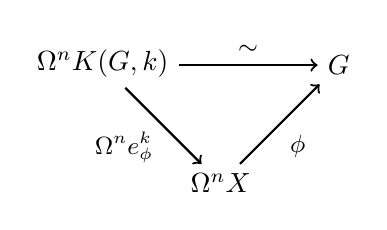
\begin{tikzpicture}[auto,node distance=2cm,
        thick,main node/.style={font=\sffamily\bfseries},text height=1.5ex]
      \node[main node] (OK) at (0,0) {$\Omega^nK(G,k)$};
      \node[main node] (G)  at (3,0) {$G$};
      \node[main node] (OX) at (1.5,-1.5) {$\Omega^n X$};
           \path[every node/.style={font=\sffamily\small}]
           (OK) edge [->] node {$\sim$} (G)
                edge [->] node [below left] {$\Omega^n e_\phi^k$} (OX)
           (OX) edge [->] node [below right] {$\phi$} (G);
    \end{tikzpicture}
  \end{center}
  Now if $\phi$ is a group isomorphism, by Whitehead's Theorem for truncated types \cite[Theorem 8.8.3]{TheBook} we know that $e_\phi^k$ is an equivalence, since it induces an equivalence on all homotopy groups (trivially on the levels other than $k$). We can also show that $e_\phi^k$ is natural in $\phi$.

  Note that if we have a group homomorphism $\psi:G\to G'$, we also get a group homomorphism $G\to\Omega^k K(G',k)$, and by the above construction we get a pointed map $K(\psi,k):K(G,k)\to_\pt K(G',k)$. This is functorial, which follows from naturality of $e_\phi^k$. 

  Finally, we can construct the equivalence explicitly. We have a functor
  $\pi_k:(0,k)\GType \to \AbGroup$ which sends $G$ to $\pi_k BG$. Conversely, we have the functor $K({-},k):\AbGroup\to (0,k)\GType$. We have natural isomorphisms
  $\pi_k K(G,k)\equiv G$ by~\autoref{thm:EM-spaces} and $K(\pi_k X,k)\equiv_\pt X$ by the application of Whitehead described above. The construction is exactly the same for $k=1$ after replacing $\AbGroup$ by $\Group$.
\end{proof}

\section{Stabilization}
\label{sec:stabilization}

In this section we discuss some constructions with higher groups~\cite{BaezDolan1998}. We will give the actions on the carriers and the deloopings, but we omit the third component, the pointed equivalence, for readability. We recommend keeping \autoref{tab:periodic} in mind during these constructions.
\begin{description}
\item[decategorification] $\Decat : (n,k)\GType \to (n-1,k)\GType$\\
  $\angled{G,B^kG} \mapsto \angled{\trunc{n-1}{G}, \trunc{n+k-1}{B^kG}}$
\item[discrete categorification] $\Disc : (n,k)\GType \to (n+1,k)\GType$ \\
  $\angled{G,B^kG} \mapsto \angled{G,B^kG}$
\end{description}
These functors make $(n,k)\GType$ a reflective sub-$(\infty,1)$-category of $(n+1,k)\GType$. That is, there is an adjunction ${\Decat} \dashv {\Disc}$. These properties are straightforward consequences of the universal property of truncation.

There are also iterated versions of these functors.
\begin{description}
  \item[$\infty$-decategorification] $\iDecat : (\infty,k)\GType \to (n,k)\GType$\\
    $\angled{G,B^kG} \mapsto \angled{\trunc{n}{G}, \trunc{n+k}{B^kG}}$
  \item[discrete $\infty$-categorification] $\iDisc : (n,k)\GType \to (\infty,k)\GType$ \\
    $\angled{G,B^kG} \mapsto \angled{G,B^kG}$
\end{description}
These functors satisfy the same properties: ${\iDecat} \dashv {\iDisc}$ such that the counit induces an isomorphism ${\iDecat} \circ {\iDisc} = \idfunc$.

For the next constructions, we need the following properties.
\begin{defn}
  For $A : \UU_\pt$ we define the \emph{$n$-connected cover} of $A$ to be 
  $A{\angled n} := \fib(A \to \trunc{n}{A})$. We have the projection $p_1: A{\angled n} \to_\pt A$.
\end{defn}
\begin{lem} \label{lem:connected-cover-univ}
  The universal property of the $n$-connected cover states the following. For any $n$-connected pointed type $B$, the pointed map
  $$(B \to_\pt A{\angled n}) \to_\pt (B \to_\pt A),$$
  given by postcomposition with $p_1$, is an equivalence.\\
\end{lem}
\begin{proof}
  Given a map $f:B\to_\pt A$, we can form a map $\widetilde f: B \to A{\angled n}$. First note that for $b:B$ the type $\tr{fb}_n=_{\trunc{n}{A}}\tr{\pt}_n$ is $(n-1)$-truncated and inhabited for $b=\pt$. Since $B$ is $n$-connected, the universal property for connected types shows that we can construct a $qb:\tr{fb}_n=\tr{\pt}_n$ for all $b$ such that $q_0:qb_0\cdot\mathsf{ap}_{\tr{\blank}_n}(f_0)=1$. Then we can define the map $\widetilde f(b):=(fb, qb)$. Now $\widetilde f$ is pointed, because $(f_0,q_0):(fb_0,qb_0)=(a_0,1)$.

  Now we show that this is indeed an inverse to the given map. On the one hand, we need to show that if $f: B \to_\pt A$, then $\proj 1 \circ \widetilde f=f$. The underlying functions are equal because they both send $b$ to $f(b)$. They respect points in the same way, because
  $\mathsf{ap}{p_1}(\widetilde f_0)=f_0$. The proof that the other composite is the identity follows from a computation using fibers and connectivity, which we omit here, but can be found in the formalization.
\end{proof}
The next reflective sub-$(\infty,1)$-category is formed by looping and delooping.
\begin{description}
\item[looping] $\Omega : (n,k)\GType \to (n-1,k+1)\GType$ \\
  $\angled{G,B^kG} \mapsto \angled{\Omega G,B^kG{\angled k}}$
\item[delooping] $\B : (n,k)\GType \to (n+1,k-1)\GType$ \\
  $\angled{G,B^kG} \mapsto \angled{\Omega^{k-1}B^kG,B^kG}$
\end{description}
We have ${\B} \dashv {\Omega}$, which follows from Lemma \ref{lem:connected-cover-univ} %note: autoref writes "Theorem"
and $\Omega\circ{\B} = \idfunc$, which follows from the fact that $A{\angled n}=A$ if $A$ is $n$-connected.

The last adjoint pair of functors is given by stabilization and forgetting. This does not form a reflective sub-$(\infty,1)$-category.
\begin{description}
\item[forgetting] $F : (n,k)\GType \to (n,k-1)\GType$ \\
  $\angled{G,B^kG} \mapsto \angled{G,\Omega B^kG}$
\item[stabilization] $S : (n,k)\GType \to (n,k+1)\GType$ \\
  $\angled{G,B^kG} \mapsto \angled{SG,\trunc{n+k+1}{\susp B^kG}}$,\\
  where $SG = \trunc{n}{\Omega^{k+1}\susp B^kG}$
\end{description}
We have the adjunction ${S} \dashv {F}$ which follows from the suspension-loop adjunction $\Sigma\dashv\Omega$ on pointed types.

The next main goal in this section is the stabilization theorem,
stating that the ditto marks in~\autoref{tab:periodic} are justified.

The following corollary is almost \cite[Lemma~8.6.2]{TheBook}, but
proving this in Book HoTT is a bit tricky. See the
formalization for details.
\begin{lem}[Wedge connectivity]
  \label{lem:wedge-connectivity}
  If $A : \UU_\pt$ is $n$-connected and $B: \UU_\pt$ is
  $m$-connected, then the map $A \vee B \to A \times B$ is
  $(n+m)$-connected.
\end{lem}

Let us mention that there is an alternative way to prove the wedge
connectivity lemma: Recall that if $A$ is $n$-connected and $B$ is
$m$-connected, then $A \ast B$ is
$(n+m+2)$-connected~\cite[Theorem~6.8]{joinconstruction}. Hence the
wedge connectivity lemma is also a direct consequence of the following lemma.
\begin{lem}
Let $A$ and $B$ be pointed types.
The fiber of the wedge inclusion $A\vee B\to A\times B$ is equivalent to
$\Omega{A}\ast\Omega{B}$. 
\end{lem}
\begin{proof}
Note that the fiber of $A\to A\times B$ is $\Omega B$, the fiber of $B\to A\times B$ is $\Omega A$, and of course the fiber of $1\to A\times B$ is $\Omega A\times \Omega B$. We get a commuting cube
\begin{equation*}
\begin{tikzcd}
& \Omega A\times \Omega B \arrow[dl] \arrow[d] \arrow[dr] \\
\Omega B \arrow[d] & 1 \arrow[dl] \arrow[dr] & \Omega A \arrow[dl,crossing over] \arrow[d] \\
A \arrow[dr] & 1 \arrow[d] \arrow[from=ul,crossing over] & B \arrow[dl] \\
& A\times B
\end{tikzcd}
\end{equation*}
in which the vertical squares are pullback squares. 

By the descent theorem for pushouts it now follows that $\Omega A\ast \Omega B$ is the fiber of the wedge inclusion.
\end{proof}

The second main tool we need for the stabilization theorem is:
\begin{thm}[Freudenthal]
  If $A : \UU_\pt^{>n}$ with $n\ge 0$, then the map
  $A \to \Omega\susp A$ is $2n$-connected.
\end{thm}
This is \cite[Theorem~8.6.4]{TheBook}.

The final building block we need is:
\begin{lem}
  There is a pullback square
  \[
    \begin{tikzcd}
      \susp\Omega A \ar[d,"\varepsilon_A"']\ar[r] & A \vee A \ar[d] \\
      A \ar[r,"\Delta"'] & A \times A
    \end{tikzcd}
  \]
  for any $A : \UU_\pt$.
\end{lem}

\begin{proof}
Note that the pullback of $\Delta:A\to A\times A$ along either inclusion $A\to A\times A$ is contractible. So we have a cube
\begin{equation*}
\begin{tikzcd}
& \Omega A \arrow[dl] \arrow[d] \arrow[dr] \\
1 \arrow[d] & 1 \arrow[dl] \arrow[dr] & 1 \arrow[dl,crossing over] \arrow[d] \\
A \arrow[dr] & A \arrow[d,"\Delta"] \arrow[from=ul,crossing over] & A \arrow[dl] \\
& A\times A
\end{tikzcd}
\end{equation*}
in which the vertical squares are all pullback squares. Therefore, if we pull back along the wedge inclusion, we obtain by the descent theorem for pushouts that the square in the statement is indeed a pullback square.
\end{proof}

\begin{thm}[Stabilization]
  \label{thm:stabilization}
  If $k\ge n+2$, then $S : (n,k)\GType \to (n,k+1)\GType$ is an
  equivalence, and any $G : (n,k)\GType$ is an infinite loop space.
\end{thm}
\begin{proof}
  We show that $F\circ S=\idfunc=S\circ F : (n,k)\GType \to (n,k)\GType$
  whenever $k\ge n+2$.

  For the first, the unit map of the adjunction factors as
  \[
    B^kG \to \Omega\susp B^kG \to \Omega\trunc{n+k+1}{\susp B^kG}
  \]
  where the first map is $2k-2$-connected by Freudenthal, and the
  second map is $n+k$-connected. Since the domain is $n+k$-truncated,
  the composite is an equivalence whenever $2k-2 \ge n+k$.

  For the second, the counit map of the adjunction factors as
  \[
    \trunc{n+k}{\susp\Omega B^kG} \to \trunc{n+k}{B^kG} \to B^kG,
  \]
  where the second map is an equivalence. By the two lemmas above, the
  first map is $2k-2$-connected.
\end{proof}
For example, for $G : (0,2)\GType$ an abelian group, we have
$B^nG = K(G,n)$, an Eilenberg-MacLane space.

The adjunction ${S} \dashv {F}$ implies that the free group on a
pointed set $X$ is $\Omega\trunc{1}{\susp X}=\pi_1(\susp X)$.  If $X$
has decidable equality, $\susp X$ is already $1$-truncated. It is an
open problem whether this is true in general.

Also, the abelianization of a set-level group $G : 1\mathsf{Grp}$ is
$\pi_2(\susp BG)$. If $G : (n,k)\GType$ is in the stable range ($k \ge
n+2$), then $SFG=G$.

\section{Perspectives on ordinary group theory}
\label{sec:perspectives}

In this section we shall indicate how the theory of higher groups can
yield a new perspective even on ordinary group theory.

From the symmetric groups $\Sym_n$, we can get other finite groups using
the constructions of~\autoref{sec:elementary-constructions}. Other
groups can be constructed more directly. For example,
$BA_n$, the classifying type of the alternating group, can be taken to
be the type of $n$-element sets $X$ equipped with a \emph{sign
  ordering}: this is an equivalence class of an ordering
$\Fin n \equiv X$ modulo even permutations. Indeed, there are only two
possible sign orderings, so this definition corresponds to
first considering the short exact sequence
\[
  1 \to A_n \to \Sym_n \xrightarrow{\mathrm{sgn}}{} \Sym_2 \to 1
\]
where the last map is the sign map, then realizing the sign map
as given by the map $\mathrm{Bsgn} : \BS_n \to \BS_2$ that takes
an $n$-element set to its set of sign orderings, and finally
letting $BA_n$ be the homotopy fiber of $\mathrm{Bsgn}$.

Similarly, $BC_n$, the classifying type of the cyclic group on $n$
elements, can be taken to be the type of $n$-elements sets $X$
equipped with a \emph{cyclic ordering}: an equivalence class of an
ordering $\Fin n \equiv X$ modulo cyclic permutations. But unlike
the above, where we had the coincidence that $\Aut(\Sym_2) \equiv
\Sym_2$,
this doesn't correspond to a short exact sequence. Rather,
it corresponds to a sequence
\[
  1 \to C_n \to \Sym_n \to \Aut(\Fin(n-1)) \equiv \Sym_{(n-1)!}
\]
where the delooping of the last map is the map from $\BS_n$ to
$\BS_{(n-1)!}$ that maps an $n$-element set to the set of cyclic
orderings, of which there are $(n-1)!$ many -- since once we fix the
position in the ordering of a particular element,
we are free to permute the rest.

As another example,
consider the map $p : \BS_4 \to_\pt \BS_3$ that maps a 4-element set
$X$ to its set of 2-by-2 partitions, of which there $3$. Using this
construction, we can realize some famous semidirect and wreath product identities,
such as $A_4 \equiv S_2^2 \rtimes A_3$, $S_4 \equiv S_2^2 \rtimes
S_3$, and, for the octahedral group, $O_h \equiv S_2^3 \rtimes S_3
\equiv S_2 \wr S_3$.

\smallskip

Let us turn to a different way of getting new groups from old, namely
via covering space theory.

\subsection{\texorpdfstring{$1$}{1}-groups and covering spaces}
\label{sec:covering}

The connection between covering spaces of a pointed connected type
$X$ and sets with an action of the fundamental group of $X$ has
already been established in homotopy type
theory~\cite{FavoniaHarper2016}. Let us recall this connection and
expand a bit upon it.

For us, a pointed connected type $X$ is equivalently
an $\infty$-group $G:\infty\mathsf{Grp}$
with delooping $BG := X$.
A covering space over $BG$ is simply a type family $C : BG \to \mathsf{Set}$
that lands in the universe of sets.
Hence by our discussion of actions in~\autoref{sec:actions}
it is precisely a set with a $G$-action.
Since $\mathsf{Set}$ is a 1-type, $C$ extends uniquely to a type family
$C' : \trunc{1}{BG} \to \mathsf{Set}$,
but $\trunc{1}{BG}$ is the delooping of the fundamental group
of $X$, and hence $C'$ is the uniquely determined
choice of a set with an action of the fundamental group.

The universal covering space is the simply connected cover of $BG$,
\[
  \widetilde{BG} : BG \to \mathsf{Set}, \quad
  z \mapsto \trunc{0}{\pt = z}.
\]
Note that the total space of $\widetilde{BG}$ is indeed the
$1$-connected cover $BG\angled1$,
since $\trunc{0}{\pt =_{BG} \pt} \equiv (\tr{\pt} =_{\trunc{1}{BG}} \tr{\pt})$.
Also note that if $G$ is already a 1-group, then this is just the right
action of $G$ on itself, and in general, it is the right action of $G$
on the fundamental group
(i.e., the decategorification of $G$)
via the truncation homomorphism from $G$ to $\pi_1(BG)$,
where we can also view $\pi_1(BG)$ as the $1\mathsf{Grp}$ decategorification
of $G$.

In general, there is a Galois correspondence between connected covers
of $BG$ and conjugacy classes of subgroups of the fundamental group.
Indeed, if $C : BG \to \mathsf{Set}$ has a connected total space,
then the space $(g : \trunc{1}{BG}) \times C'(g)$
is itself a connected, 1-truncated type,
and the projection to $\trunc{1}{BG}$
induced an inclusion of fundamental groups
once a point $\pt : C'(\pt)$ has been chosen.

\begin{thm}[Fundamental theorem of Galois theory for covering spaces]
  \label{thm:galois-zero}
  $\phantom{42}$
  \begin{enumerate}
  \item  The automorphism group of the universal covering space
    $\widetilde{BG}$ is isomorphic to
    the $1$-group decategorification of $G$,
    \[
      \Aut(\widetilde{BG}) \equiv \Decat_1(G) \equiv \pi_1(BG).
    \]
  \item Furthermore, there is a contravariant correspondence between
    conjugacy classes of subgroups of $\Decat_1(G)$ and connected
    covers of $BG$.
  \item This lifts to a Galois correspondence between subgroups of
    $\Decat_1(G)$ and pointed, connected covers of $BG$.  The normal
    subgroups correspond to Galois covers.
  \end{enumerate}
\end{thm}
Note that the universal covering space
and the trivial covering space
(constant at the unit type)
are canonically pointed,
reflecting the fact that
the two trivial subgroups are normal.

The first part of the fundamental theorem has a clear generalization to
higher groups:
\begin{thm}[Fundamental theorem of Galois theory for $n$-covers,
  part one]
  The automorphism group of the universal $n$-type cover $U_n(BG)$,
  \[
    U_n(BG) : BG \to \UU^{\le n},
    \quad
    z \mapsto \trunc{n}{\pt = z}
  \]
  of $BG$ is
  isomorphic to the $(n+1)$-group decategorification of $G$,
  \[
    \Aut(U_n(BG)) \equiv \Decat_{n+1}(G) \equiv \Pi_{n+1}(BG).
  \]
\end{thm}
\begin{proof}
  Note that
  $\BAut(U_n(BG))$ is the image of the map $1 \to (BG \to \UU^{\le
    n})$ that sends the canonical element to $U_n(BG)$. Since $BG$ is
  connected, this image is exactly $\trunc{n+1}{BG}$ by
  \cite[Theorem~7.1]{joinconstruction}. Then we are done,
  since $\B\Pi_{n+1}(BG) \equiv \trunc{n+1}{BG}$, by definition.
\end{proof}
It is possible to use the other parts
of~\autoref{thm:galois-zero} in order to \emph{define} the notions of
subgroup and normal subgroup for $n$-groups, which then become
\emph{structure on} rather than a \emph{property of} a homomorphism $f
: K \to G$.
Explicitly, the structure of a \emph{normal subgroup} on such an $f$
is a delooping $B(G \dblslash K)$ of the type $G \dblslash K$
together with a map $Bq : BG \to_\pt B(G \dblslash K)$ giving rise to a
fiber sequence
\begin{equation}\label{eq:normal-fiber-sequence}
  G \dblslash K \to BK \xrightarrow{Bf}{} BG
  \xrightarrow{Bq}{} B(G \dblslash K).
\end{equation}

\subsection{Central extensions and group cohomology}
\label{sec:group-cohomology}

The cohomology of a higher group $G$ is simply the cohomology of its
delooping $BG$. Indeed, for any spectrum $A$, we define
\[
  H_{\mathrm{Grp}}^k(G, A) := \trunc{0}{BG \to_\pt B^kA}.
\]
Of course, to define the $k$'th cohomology group, we only need the
$k$-fold delooping $B^kA$.

If $A:(\infty,2)\GType$ is a braided $\infty$-group, then
we have the second cohomology group $H_{\mathrm{Grp}}^2(G, A)$, and an
element $c:BG \to_\pt B^2A$ gives rise to a \emph{central extension}
\[
  BA \to BH \to BG \xrightarrow{c}{} B^2A,
\]
where $BH$ is the homotopy fiber of $c$.  This lifts to the world of
higher groups the usual result that isomorphism classes of central
extensions of a $1$-group $G$ by an abelian $1$-group $A$
are given by cohomology classes in $H_{\mathrm{Grp}}^2(G, A)$.

\smallskip

In the Spectral repository there is full formalization of the Serre
spectral sequence for cohomology \cite{SerreSpectralSequence}.
If we have any normal subgroup fiber sequence for $\infty$-groups as
in~\eqref{eq:normal-fiber-sequence}, then we get a corresponding
spectral sequence with $E_2$-page
\[
  H_{\mathrm{Grp}}^p(G \dblslash K, H_{\mathrm{Grp}}^q(K, A))
\]
and converging to $H_{\mathrm{Grp}}^n(G, A)$, where $A$ is any
truncated, connective spectrum, which could even be a left $G$-module,
in which case we reproduce the \emph{Hochschild-Serre spectral
  sequence}.
